\chapter{SYSTEM DESIGN}

\section{Project Design}
System design is the process of defining the architecture, components, modules, interfaces, and data for a system to satisfy specified requirements. In ParkX, the design architecture is built around an MVC (Model-View-Controller) structure, specifically customized to support high-concurrency parking operations with atomic transactional hold times.

\subsection{Consolidated System Diagrams}
As per the project requirements, all foundational architectural and logical diagrams are consolidated below to provide a unified overview of the system's design.

\vspace{1cm}
\begin{figure}[H]
    \centering
    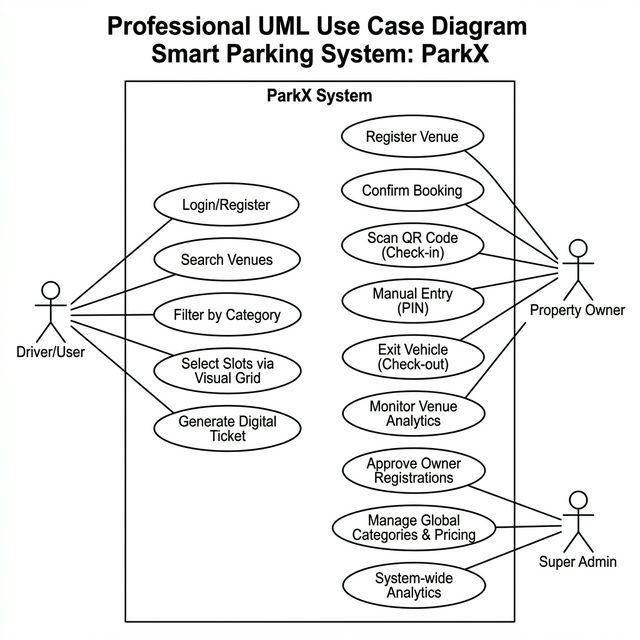
\includegraphics[width=0.9\textwidth]{diag_use_case.png}
    \caption{UML Use Case Diagram - System Boundary \& Actors}
    \label{fig:use_case}
\end{figure}
\vspace{1cm}

\vspace{1cm}
\begin{figure}[H]
    \centering
    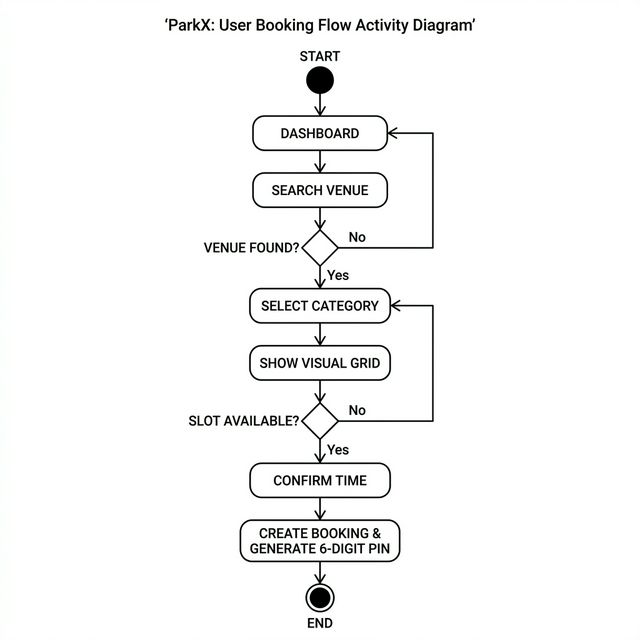
\includegraphics[width=0.9\textwidth]{diag_activity_booking.png}
    \caption{Activity Diagram - User Booking Flow}
    \label{fig:activity}
\end{figure}
\vspace{1cm}


\begin{figure}[H]
    \centering
    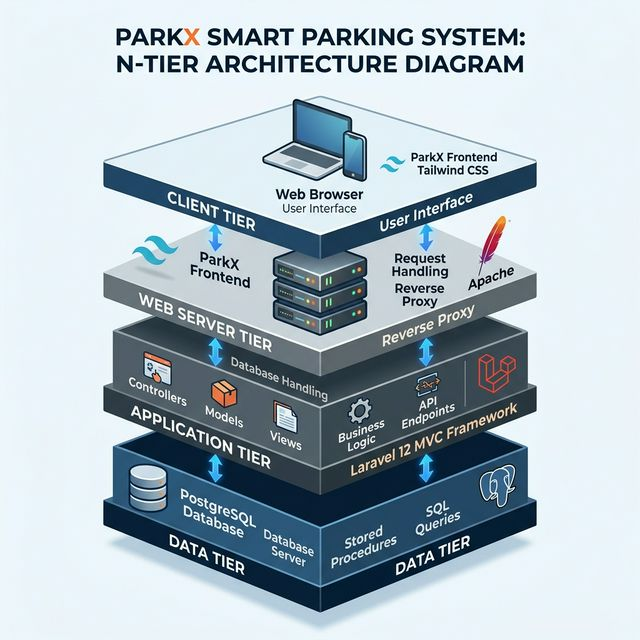
\includegraphics[width=0.9\textwidth]{diag_system_architecture.png}
    \caption{System Architecture Diagram}
    \label{fig:architecture}
\end{figure}
\vspace{1cm}

\vspace{1cm}
\begin{figure}[H]
    \centering
    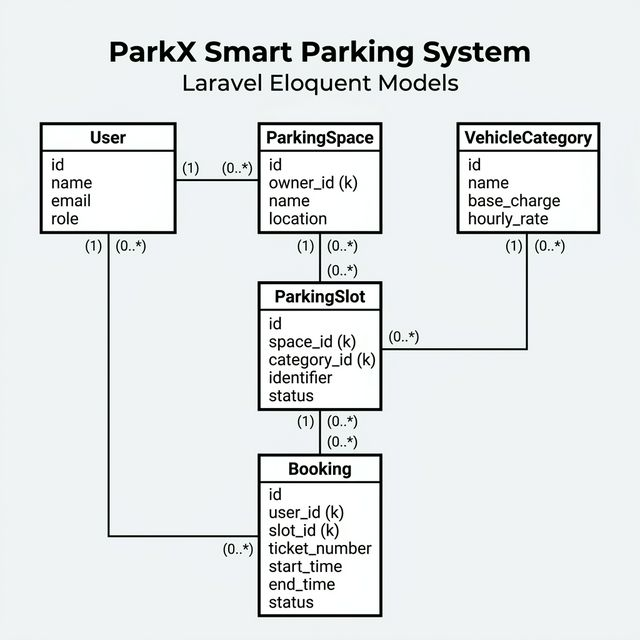
\includegraphics[width=0.9\textwidth]{diag_class_diagram_models.png}
    \caption{UML Class Diagram - Eloquent Models}
    \label{fig:class}
\end{figure}
\vspace{1cm}

\vspace{1cm}
\begin{figure}[H]
    \centering
    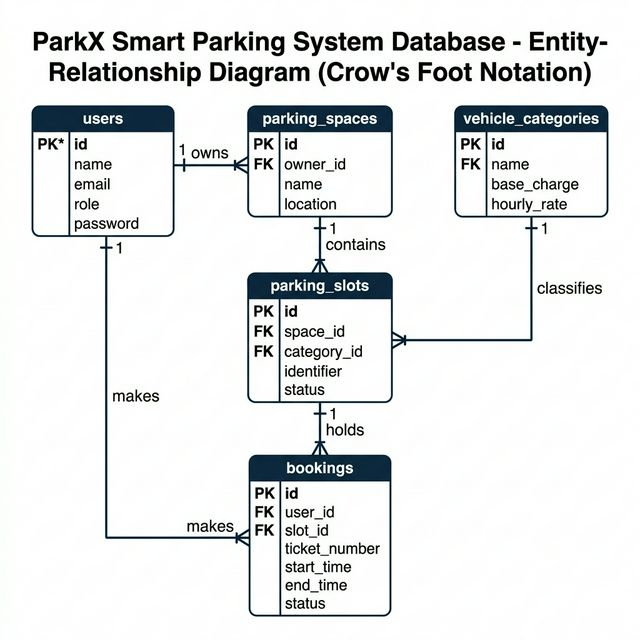
\includegraphics[width=0.9\textwidth]{diag_er_diagram_schema.png}
    \caption{Entity-Relationship (ER) Diagram}
    \label{fig:er}
\end{figure}
\vspace{1cm}

\vspace{1cm}
\begin{figure}[H]
    \centering
    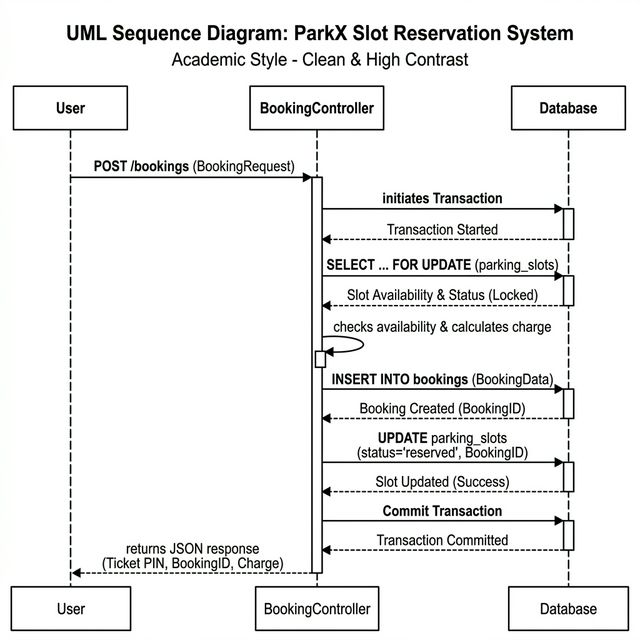
\includegraphics[width=0.9\textwidth]{diag_sequence_locking.png}
    \caption{Sequence Diagram (Transactional Slot Locking)}
    \label{fig:sequence}
\end{figure}
\vspace{1cm}

\begin{figure}[H]
    \centering
    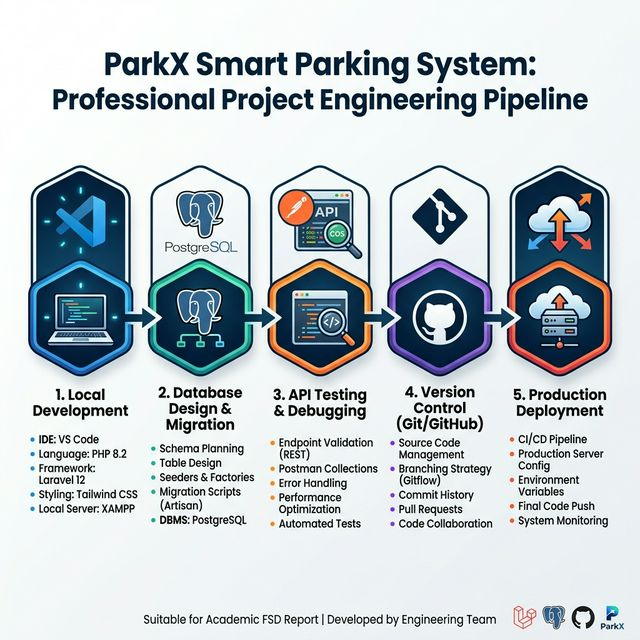
\includegraphics[width=0.9\textwidth]{diag_project_pipeline.png}
    \caption{Project Pipeline}
    \label{fig:pipeline}
\end{figure}
\vspace{1cm}

\section{User Interface (UI) Design}
The user interface of ParkX adheres to the "Antigravity" design blueprint, which emphasizes minimalism, depth, and smooth interactions.

\subsection{Design Aesthetics}
The interface utilizes semi-transparent glassmorphism elements, vibrant gradients, and high-contrast typography (Inter/Oswald) to create a premium, modern feel. Micro-interactions and subtle transitions are employed to provide immediate feedback to the driver or property owner.

\subsection{UI Review (Screenshots)}
The following represent the core interface screens of the ParkX application:

\vspace{0.5cm}
[INSERT IMAGE HERE: Figure 4.8 - Landing Page UI]
\vspace{0.5cm}

\vspace{0.5cm}
[INSERT IMAGE HERE: Figure 4.9 - Authentication Portal]
\vspace{0.5cm}

\vspace{0.5cm}
[INSERT IMAGE HERE: Figure 4.10 - Super Admin Dashboard]
\vspace{0.5cm}

\vspace{0.5cm}
[INSERT IMAGE HERE: Figure 4.11 - Owner Management Hub]
\vspace{0.5cm}

\vspace{0.5cm}
[INSERT IMAGE HERE: Figure 4.12 - User Booking Interface with Slot Grid]
\vspace{0.5cm}

\section{Database Design}
ParkX utilizes a highly normalized relational database implemented in \textbf{PostgreSQL}. The schema is designed to ensure referential integrity while supporting the high-concurrency needs of real-time slot selection.

\newpage
\subsection{Core Entity Tables}

\paragraph{Table: \textbf{users}}
Stores authentication, identification, and role-based credentials.
\begin{longtable}{|p{3cm}|p{3cm}|p{2cm}|p{6cm}|}
    \hline
    \textbf{Attribute} & \textbf{Data Type} & \textbf{Key} & \textbf{Description} \\
    \hline
    \endhead
    id & BigSerial & PK & Primary unique identifier \\
    \hline
    name & Varchar(255) & - & Full name of the user \\
    \hline
    email & Varchar(255) & Unique & Login email address \\
    \hline
    role & Varchar(20) & - & Roles: 'admin', 'owner', 'user' \\
    \hline
    password & Varchar(255) & - & Bcrypt hashed password \\
    \hline
\end{longtable}

\paragraph{Table: \textbf{vehicle\_categories}}
Maintains the global taxonomy of vehicle types and their associated pricing logic.
\begin{longtable}{|p{3cm}|p{3cm}|p{2cm}|p{6cm}|}
    \hline
    \textbf{Attribute} & \textbf{Data Type} & \textbf{Key} & \textbf{Description} \\
    \hline
    \endhead
    id & BigSerial & PK & Unique category ID \\
    \hline
    name & Varchar(255) & - & E.g., 'Two Wheeler' \\
    \hline
    base\_charge & Decimal(8,2) & - & Flat entry fee \\
    \hline
    hourly\_rate & Decimal(8,2) & - & Incremental cost per hour \\
    \hline
\end{longtable}

\subsection{Inventory and Infrastructure Tables}

\paragraph{Table: \textbf{parking\_spaces}}
Represents physical venues managed by owners.
\begin{longtable}{|p{3cm}|p{3cm}|p{2cm}|p{6cm}|}
    \hline
    \textbf{Attribute} & \textbf{Data Type} & \textbf{Key} & \textbf{Description} \\
    \hline
    \endhead
    id & BigSerial & PK & Unique venue ID \\
    \hline
    owner\_id & BigInt & FK & References \textbf{users.id} \\
    \hline
    name & Varchar(255) & - & Venue name \\
    \hline
    location & Text & - & Physical GIS/Address details \\
    \hline
\end{longtable}

\paragraph{Table: \textbf{parking\_slots}}
The atomic unit of inventory within a parking space.
\begin{longtable}{|p{3cm}|p{3cm}|p{2cm}|p{6cm}|}
    \hline
    \textbf{Attribute} & \textbf{Data Type} & \textbf{Key} & \textbf{Description} \\
    \hline
    \endhead
    id & BigSerial & PK & Unique slot ID \\
    \hline
    space\_id & BigInt & FK & References \textbf{parking\_spaces.id} \\
    \hline
    category\_id & BigInt & FK & References \textbf{vehicle\_categories.id} \\
    \hline
    identifier & Varchar(50) & - & E.g., 'A1', 'P-04' \\
    \hline
    status & Enum & - & 'available', 'occupied', 'reserved' \\
    \hline
\end{longtable}

\subsection{Transactional Tables}

\paragraph{Table: \textbf{bookings}}
Logs the orchestration between users and reserved slots.
\begin{longtable}{|p{3cm}|p{3cm}|p{2cm}|p{6cm}|}
    \hline
    \textbf{Attribute} & \textbf{Data Type} & \textbf{Key} & \textbf{Description} \\
    \hline
    \endhead
    id & BigSerial & PK & Unique booking ID \\
    \hline
    user\_id & BigInt & FK & References \textbf{users.id} \\
    \hline
    slot\_id & BigInt & FK & References \textbf{parking\_slots.id} \\
    \hline
    ticket\_number & Varchar(6) & Unique & Manual fallback PIN code \\
    \hline
    start\_time & Timestamp & - & Scheduled entry time \\
    \hline
    end\_time & Timestamp & - & Scheduled exit time \\
    \hline
    scanned\_at & Timestamp & - & Actual check-in timestamp \\
    \hline
    status & Varchar(20) & - & 'booked', 'occupied', 'completed' \\
    \hline
\end{longtable}
